\documentclass[conference]{IEEEtran}
\IEEEoverridecommandlockouts
\usepackage{cite}
\usepackage{amsmath,amssymb,amsfonts}
\usepackage{graphicx}
\usepackage{textcomp}
\usepackage{xcolor}
\usepackage{booktabs}
\usepackage{multirow}
\usepackage{url}
\graphicspath{{figures/}}

% Visible placeholder for facts only the authors can supply. Resolve all before submission:
%   grep -n authortodo main.tex
\newcommand{\authortodo}[1]{\textcolor{red}{\textbf{[TODO: #1]}}}

\begin{document}

\title{Does Hybridization Help? A Leakage-Free, Subject-Level Benchmark of 3D CNN, Transformer, and Hybrid Models for Alzheimer's Disease Classification from Structural MRI}

\author{
\IEEEauthorblockN{Pinky Akter, Samuel Emon Halder, Md. Sarjil Hasan, A.S. Zaforullah Momtaz, Faria Zarin Subah}
\IEEEauthorblockA{Department of Computer Science and Engineering, University of Asia Pacific, Dhaka, Bangladesh\\
\authortodo{author e-mail addresses; confirm author order}}
}

\maketitle

\begin{abstract}
Many deep-learning studies of Alzheimer's disease (AD) report near-perfect accuracy from structural MRI, but they often split data at the level of 2D slices, so slices of the same patient appear in both training and test sets. We present a leakage-free benchmark of fully three-dimensional models on 1{,}132 T1-weighted MRI volumes from 395 subjects of the Alzheimer's Disease Neuroimaging Initiative (ADNI). All models share one preprocessing pipeline, one classifier head, and identical subject-level five-fold splits. We compare a 3D DenseNet-121, a MedicalNet-pretrained 3D ResNet-18, a 3D Vision Transformer (ViT), a Swin Transformer encoder, and two late-fusion hybrids (CNN--ViT and Swin--ViT) on cognitively normal (CN) vs.\ AD and CN vs.\ mild cognitive impairment (MCI) vs.\ AD classification. The CNN--ViT hybrid reaches the highest binary accuracy ($82.2\pm5.7\%$, macro-F1 $0.80$) but is statistically indistinguishable from the from-scratch DenseNet ($81.0\%$; paired $p\approx0.54$); the hybrid without a convolutional branch is far weaker ($70.2\%$). In the three-class task the best model (Swin, $57.7\%$) is only about five points above the majority-class baseline, and MCI is the main source of error. A from-scratch ViT fails to learn. A 3D attribution analysis shows that, without skull-stripping, explanation methods disagree and partly highlight non-brain tissue. The results indicate that under honest evaluation a well-trained 3D CNN is a strong baseline that transformer hybrids do not measurably improve at this data scale.
\end{abstract}

\begin{IEEEkeywords}
Alzheimer's disease, structural MRI, 3D convolutional neural network, vision transformer, data leakage, explainable AI
\end{IEEEkeywords}

\section{Introduction}
Alzheimer's disease (AD) is the most common cause of dementia, and structural MRI captures its characteristic atrophy of the hippocampus and medial temporal lobe and the resulting ventricular enlargement~\cite{scheltens2016alzheimer,frisoni2010clinical}. Deep learning has been applied widely to MRI-based AD classification, and recent work increasingly combines convolutional neural networks (CNNs), which capture local texture, with vision transformers (ViTs), which model long-range context~\cite{bravo2024systematic}.

Two problems limit what this literature tells us. First, many studies classify 2D slices and split the data at slice level, so slices of the same patient fall on both sides of the train/test boundary. Yagis \textit{et al.}~\cite{yagis2021effect} showed that such leakage raises accuracy from about 66--70\% to 95--97\% on the same data, and Wen \textit{et al.}~\cite{wen2020convolutional} found signs of leakage in more than half of the studies they reviewed. Second, hybrid CNN--transformer models are rarely compared against equally tuned single-model baselines under the same splits, so it is unclear whether fusion itself helps.

This paper addresses both problems with a controlled benchmark. Its contributions are:
\begin{itemize}
    \item A subject-level, five-fold evaluation of six fully 3D models on one curated ADNI cohort, with a shared pipeline, classifier head, and splits, and with majority-class baselines and paired statistical tests reported alongside every comparison.
    \item Evidence that a CNN--ViT hybrid does not measurably outperform a strong from-scratch 3D CNN, whereas removing the CNN branch costs about 12 accuracy points.
    \item Two documented negative results: instability of a medically pretrained ResNet, and failure of a from-scratch 3D ViT in the three-class task.
    \item A 3D explainability analysis that reports where attribution methods disagree, rather than only showing favourable maps.
\end{itemize}

\section{Related Work}
\textbf{Slice-based studies.} ViT and CNN models trained on 2D slices report 97--99.8\% accuracy for AD staging~\cite{alshayeji2024alzheimer,mahim2024unlocking,el2024novel,alsaeed2022brain}, and a CNN--Swin hybrid reaches 95.3\% on OASIS slices~\cite{velu2025design}. These pipelines either split data at slice level or use curated 2D Kaggle sets, so their figures are not comparable with subject-level results~\cite{yagis2021effect}.

\textbf{Subject-level 3D studies.} Under subject-level evaluation, reported performance is markedly lower. Wen \textit{et al.}~\cite{wen2020convolutional} obtained 85--88\% for AD vs.\ CN with 3D CNNs in a reproducible framework, and B{\"a}ckstr{\"o}m \textit{et al.}~\cite{backstrom2018efficient} showed that subject-level splitting is essential for 3D CNNs. Saoud and AlMarzouqi~\cite{saoud2024explainable} used one baseline scan per subject and an ensemble of 138 region-specific 3D ViTs, reporting 90\% for AD vs.\ CN but only 60\% for the three-class task. Our work follows this subject-level line and focuses on whether hybridization adds value over strong single models.

\section{Materials and Methods}
\subsection{Data}
We used ADNI~\cite{jack2008adni,petersen2010adni} 3T T1-weighted MPRAGE volumes (ADNI GO/2/3) in the pre-processed N3m NIfTI form. We removed 18 scans from 9 subjects that were hippocampal segmentations or followed an off-pipeline protocol; all 9 subjects kept their standard scans. Table~\ref{tab:data} summarizes the cohort. Subjects contribute 2.9 scans on average, so a subject-level split is essential.

\begin{table}[t]
\centering
\caption{Curated ADNI cohort}
\label{tab:data}
\begin{tabular}{lccc}
\toprule
Group & Subjects & Scans & Task \\
\midrule
CN  & 206 & 627 & binary, 3-class \\
MCI & 80  & 182 & 3-class \\
AD  & 109 & 323 & binary, 3-class \\
\midrule
Total & 395 & 1{,}132 & \\
\bottomrule
\end{tabular}
\end{table}

\subsection{Evaluation Protocol}
We built stratified five-fold splits at the \emph{subject} level (seed 42), so that no subject's scans appear in both training and test data; this is asserted in code. The same splits are used for every model. \authortodo{state where the validation subjects used for early stopping come from in each fold, e.g.\ an inner split of the four training folds}. Scan-level outputs are averaged per subject to give one subject-level prediction, and all metrics are computed at subject level. Because the classes are imbalanced, we use macro-F1 as the primary metric and report accuracy and weighted-F1 as secondary metrics. Always predicting CN gives the majority-class baseline: $65.4\%$ accuracy in the binary task and $52.2\%$ in the three-class task. We report mean $\pm$ population standard deviation over folds, and compare models with a paired $t$-test on fold-wise macro-F1.

\subsection{Preprocessing}
A deterministic MONAI~\cite{cardoso2022monai} pipeline reorients each volume to RAS, resamples it to 1.5\,mm isotropic spacing, crops the foreground, applies z-score normalization over non-zero voxels, and resizes it to $96^3$ (all binary runs and the three-class ViT) or $128^3$ (three-class CNN and Swin). Volumes are not skull-stripped or registered. Training-only augmentation includes random flips, affine transforms ($\pm10^\circ$), Gaussian noise and smoothing, bias field, gamma, and intensity scaling.

\subsection{Models}
All backbones expose a feature vector that feeds a shared dropout (0.2) and linear classifier head.
(i)~\textbf{DenseNet-121}~\cite{huang2017densely}: 3D, trained from scratch, 1024-D features.
(ii)~\textbf{ResNet-18} initialized with MedicalNet weights~\cite{chen2019med3d}, 512-D.
(iii)~\textbf{ViT}~\cite{dosovitskiy2021image}: hidden size 384, 6 layers, 6 heads, $16^3$ patches (216 tokens), trained from scratch.
(iv)~\textbf{Swin}: the SwinUNETR encoder~\cite{hatamizadeh2021swinunetr,liu2021swin} (feature size 48, four stages) with global average pooling.
(v)~\textbf{CNN--ViT hybrid} (Fig.~\ref{fig:arch}): DenseNet and ViT branches process the same volume, and their features are concatenated (1408-D) before the head.
(vi)~\textbf{Swin--ViT hybrid}: the same design with Swin in place of DenseNet, which acts as a control for the contribution of the CNN branch.

\begin{figure}[t]
\centering
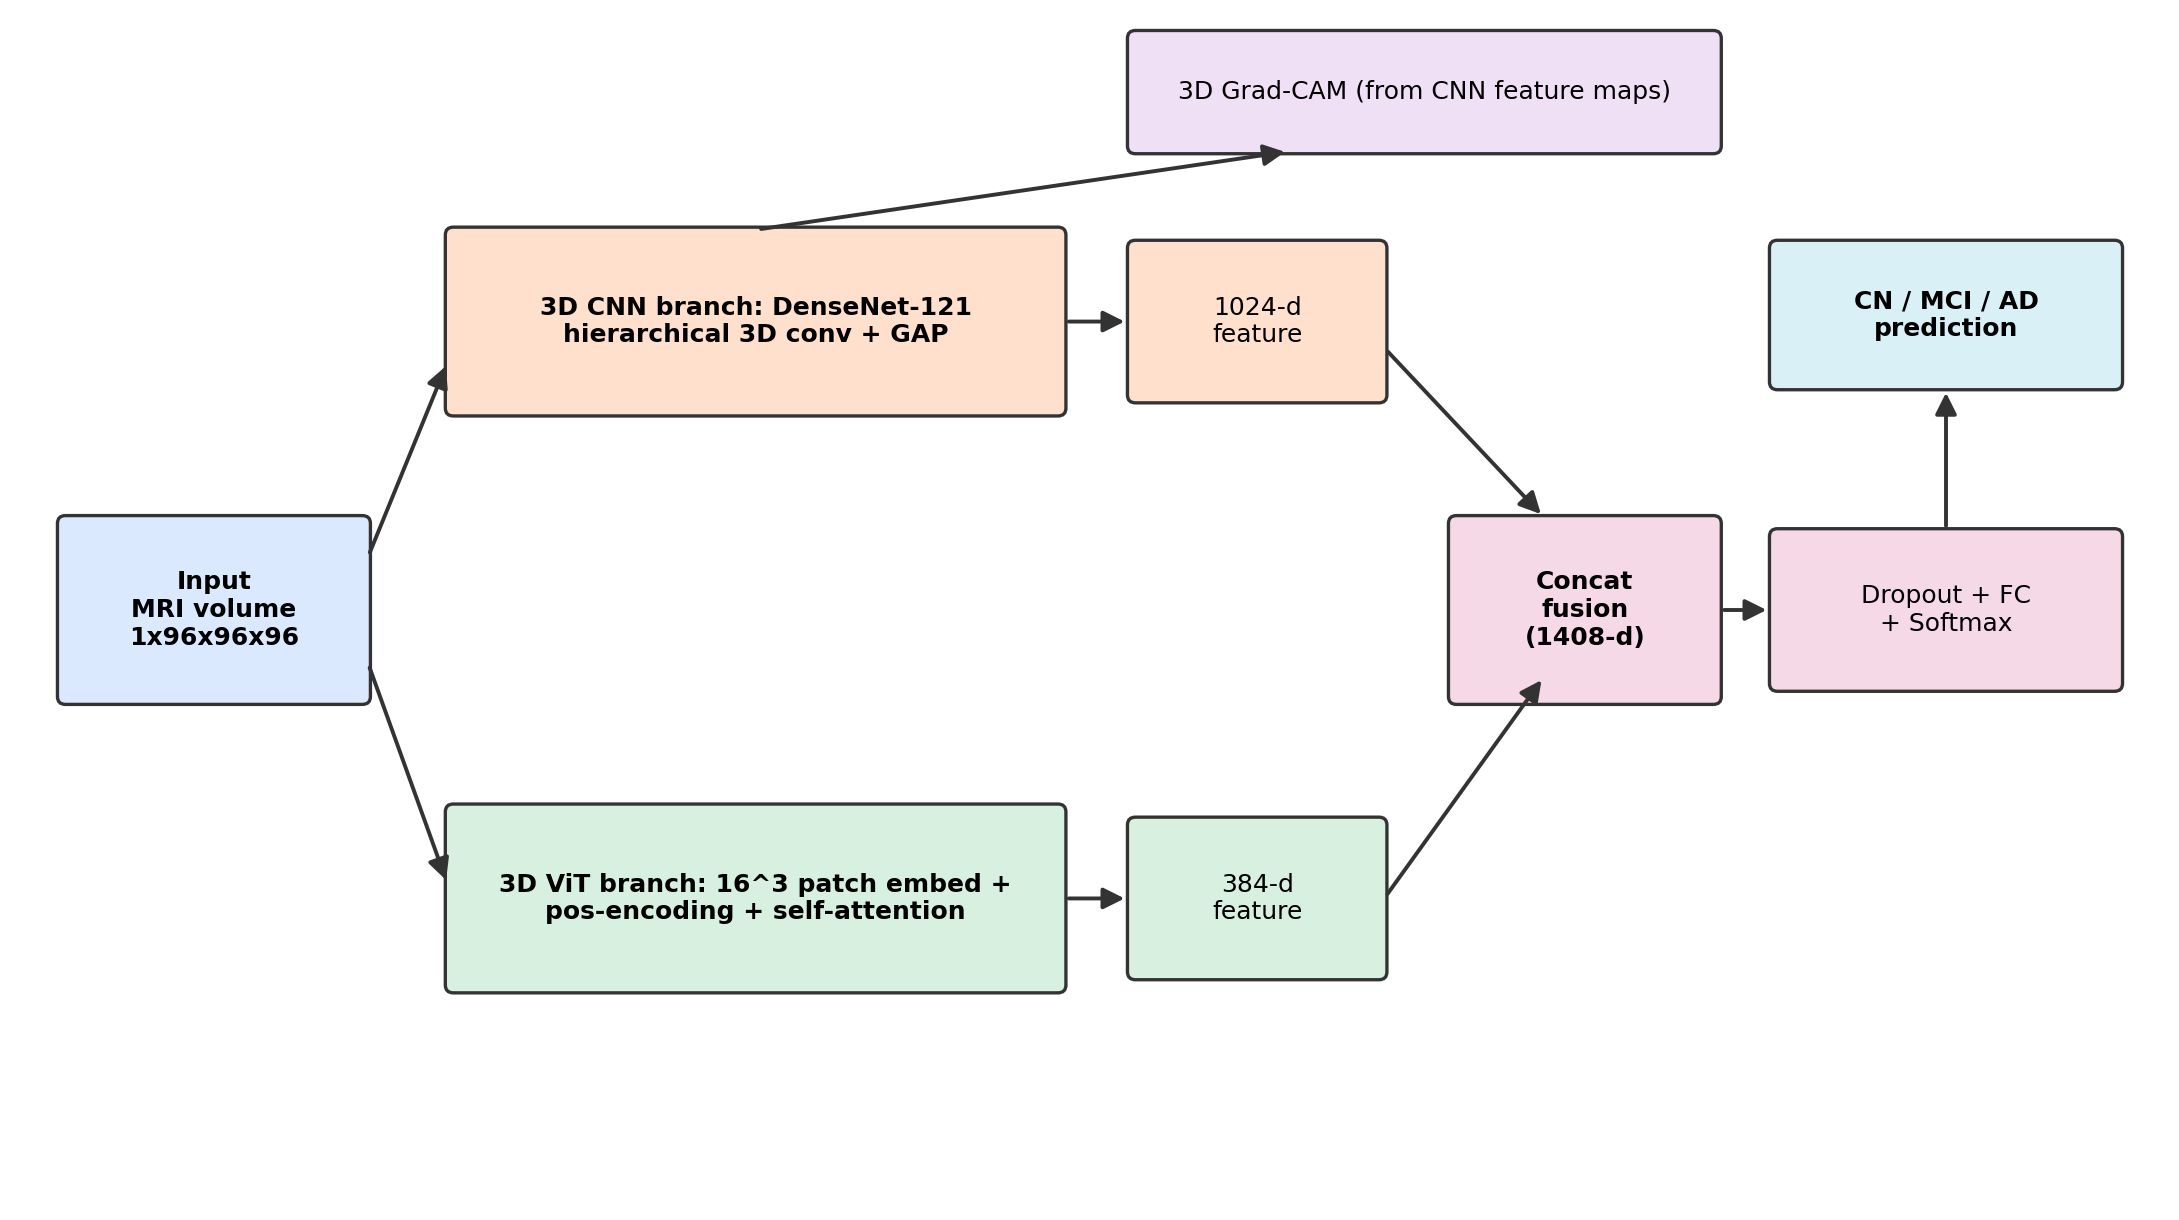
\includegraphics[width=\columnwidth]{arch_hybrid.png}
\caption{CNN--ViT hybrid. A 3D DenseNet-121 branch (local features, 1024-D) and a 3D ViT branch (global features, 384-D) process the same volume; their features are concatenated and classified by a shared dropout and linear head.}
\label{fig:arch}
\end{figure}

\begin{figure*}[t]
\centering
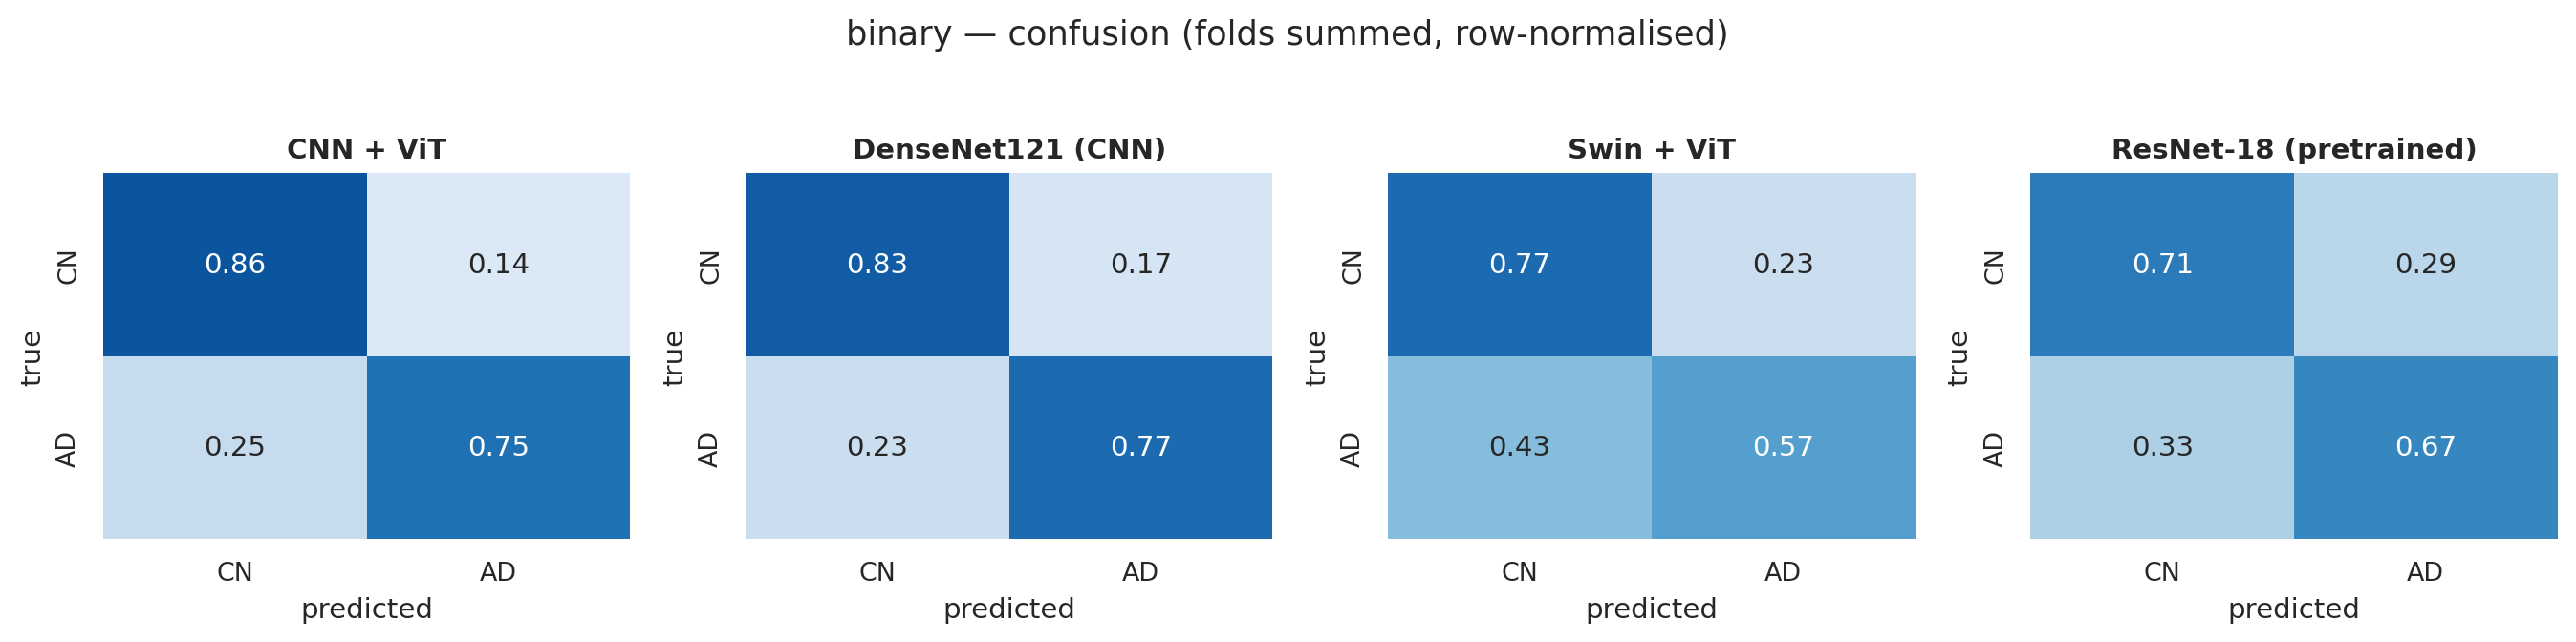
\includegraphics[width=0.85\textwidth]{res_confusion_binary.png}
\caption{Binary confusion matrices (folds summed, row-normalized, subject level).}
\label{fig:cm}
\end{figure*}

\subsection{Training}
All models use AdamW~\cite{loshchilov2019decoupled} (learning rate $10^{-4}$) with cosine decay and linear warmup, mixed precision, batch size 2 with 4-step gradient accumulation, and gradient clipping at 1.0. Binary runs use class-weighted cross-entropy with label smoothing 0.1~\cite{muller2019does}, weight decay 0.03, 8 warmup epochs, at most 100 epochs, and early-stopping patience 18. Three-class runs use focal loss~\cite{lin2017focal} ($\gamma=2$), weight decay 0.01, 5 warmup epochs, at most 80 epochs, and patience 15. \authortodo{state exactly which imbalance corrections were active per run (class weights, weighted sampler, focal loss)}. Early stopping and checkpoint selection use validation subject-level macro-F1. Training used PyTorch~\cite{paszke2019pytorch} and MONAI on one NVIDIA RTX 5060 Ti (16\,GB).

\subsection{Explainability}
For trained models we computed Grad-CAM~\cite{selvaraju2017gradcam}, Grad-CAM++~\cite{chattopadhay2018gradcampp}, Score-CAM, Integrated Gradients~\cite{sundararajan2017axiomatic}, SmoothGrad~\cite{smilkov2017smoothgrad}, occlusion, LIME~\cite{ribeiro2016why}, and, for transformers, attention rollout~\cite{abnar2020quantifying}, all in 3D.

\section{Results}
\begin{figure*}[t]
\centering
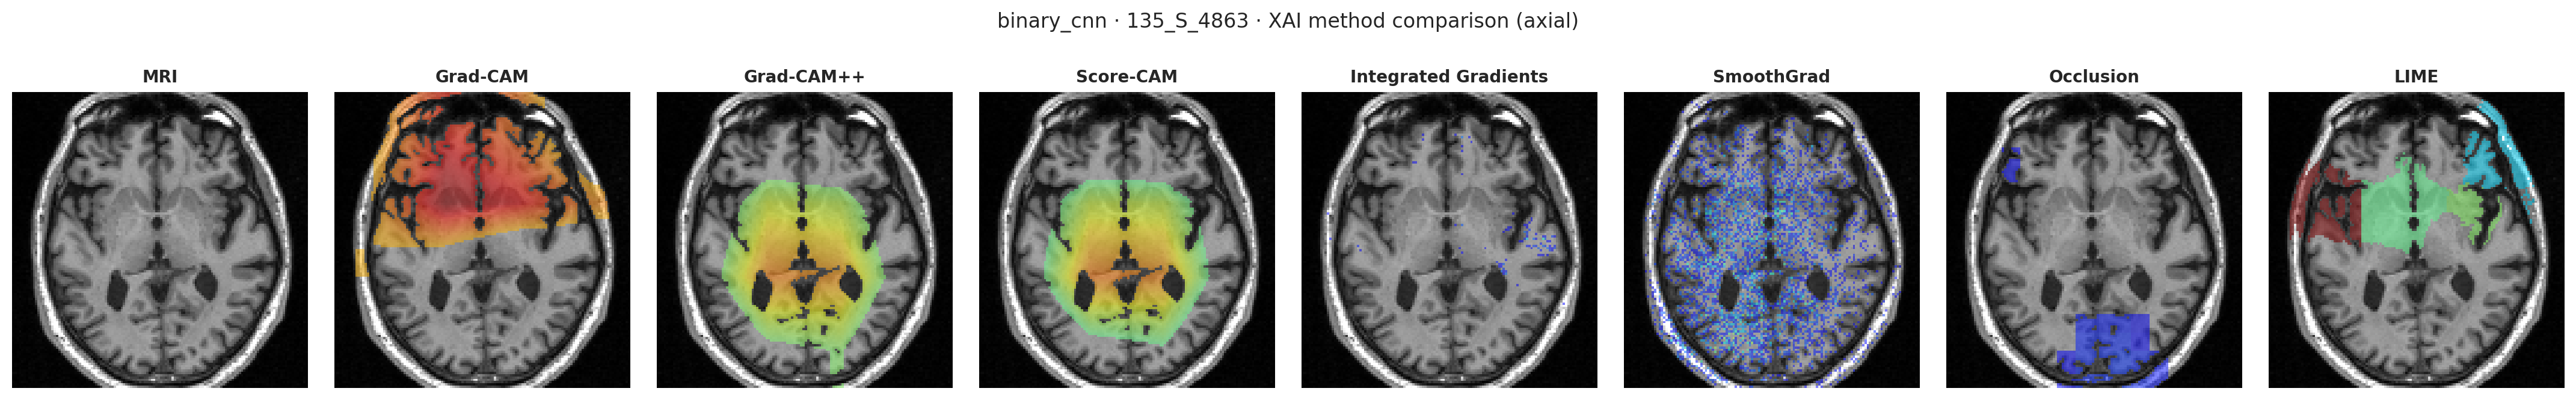
\includegraphics[width=\textwidth]{xai_panel_binary_cnn.png}
\caption{3D attribution methods for the binary DenseNet on one AD subject (axial slice). The methods highlight different regions, including non-brain tissue.}
\label{fig:xai}
\end{figure*}

\subsection{Binary CN vs.\ AD}
Table~\ref{tab:binary} reports the binary results. The CNN--ViT hybrid has the highest mean macro-F1 ($0.802$), followed closely by the from-scratch DenseNet ($0.788$). Both clearly exceed the majority-class baseline. The Swin--ViT hybrid and the pretrained ResNet are about 12 points lower in accuracy, only 4--5 points above the baseline, and much less stable across folds.

\begin{table}[t]
\centering
\caption{Binary CN vs.\ AD, subject-level 5-fold CV (mean $\pm$ SD)}
\label{tab:binary}
\setlength{\tabcolsep}{4pt}
\begin{tabular}{lccc}
\toprule
Model & Accuracy & Macro-F1 & W-F1 \\
\midrule
CNN--ViT hybrid & \textbf{0.822}$\pm$0.057 & \textbf{0.802}$\pm$0.062 & 0.820 \\
DenseNet-121 (scratch) & 0.810$\pm$0.041 & 0.788$\pm$0.062 & 0.807 \\
Swin--ViT hybrid & 0.702$\pm$0.070 & 0.662$\pm$0.101 & 0.696 \\
ResNet-18 (MedicalNet) & 0.698$\pm$0.139 & 0.654$\pm$0.168 & 0.678 \\
\midrule
\textit{Majority baseline} & \textit{0.654} & \textit{0.395} & \textit{0.517} \\
\bottomrule
\end{tabular}
\end{table}

\textbf{Is the hybrid better?} The fold-wise macro-F1 differences between the CNN--ViT hybrid and DenseNet are $-0.052$, $+0.047$, $+0.065$, $-0.013$, and $+0.023$ (mean $+0.014$). A paired $t$-test gives $t=0.67$ with 4 degrees of freedom ($p\approx0.54$). The hybrid wins three of five folds and classifies 259 of 315 subjects correctly against DenseNet's 255. We therefore find no evidence that adding the ViT branch helps. Removing the CNN branch, however, is costly: Swin--ViT loses about 14 points of macro-F1, which indicates that the convolutional branch carries most of the signal at this data scale.

Fig.~\ref{fig:cm} shows the confusion matrices. CNN--ViT and DenseNet recover both classes with balanced errors (CN recall $0.83$--$0.86$, AD recall $0.75$--$0.77$), whereas Swin--ViT misses $43\%$ of AD subjects.

\subsection{Three-Class CN vs.\ MCI vs.\ AD}
Table~\ref{tab:3class} reports the three-class results. Swin and DenseNet are tied ($t=0.70$, $p\approx0.5$) at about 57\% accuracy. This is only five points above the majority baseline, although their macro-F1 is more than twice the baseline's. The pooled per-class F1 is about $0.65$ for CN, $0.55$--$0.61$ for AD, and only $0.37$--$0.41$ for MCI; most MCI subjects are assigned to CN or AD. For DenseNet, the one-vs-rest AUCs are $0.69$ (CN), $0.66$ (MCI), and $0.77$ (AD). The CNN--ViT hybrid was not evaluated on this task.

\begin{table}[t]
\centering
\caption{Three-class CN/MCI/AD, subject-level 5-fold CV}
\label{tab:3class}
\setlength{\tabcolsep}{4pt}
\begin{tabular}{lccc}
\toprule
Model & Accuracy & Macro-F1 & W-F1 \\
\midrule
Swin & \textbf{0.577}$\pm$0.098 & \textbf{0.537}$\pm$0.078 & 0.573 \\
DenseNet-121 & 0.572$\pm$0.092 & 0.524$\pm$0.071 & 0.560 \\
ViT (scratch) & 0.286$\pm$0.015 & 0.256$\pm$0.012 & 0.184 \\
\midrule
\textit{Majority baseline} & \textit{0.522} & \textit{0.229} & \textit{0.358} \\
\bottomrule
\end{tabular}
\end{table}

\subsection{Fold Variance and Negative Results}
Fig.~\ref{fig:box} shows the fold-wise spread. The pretrained ResNet is bimodal: three folds reach $0.78$--$0.82$ macro-F1 while two fall to $0.449$. One possible explanation is that a late accuracy take-off interacts with the shared early-stopping patience, but we have not tested this. The from-scratch ViT falls \emph{below} the majority baseline in the three-class task: it never predicts CN and splits subjects between MCI and AD. This is consistent with the data demands of a ViT trained from scratch~\cite{dosovitskiy2021image}, possibly compounded by imbalance corrections that push a model that has learned nothing useful toward minority classes.

\begin{figure}[t]
\centering
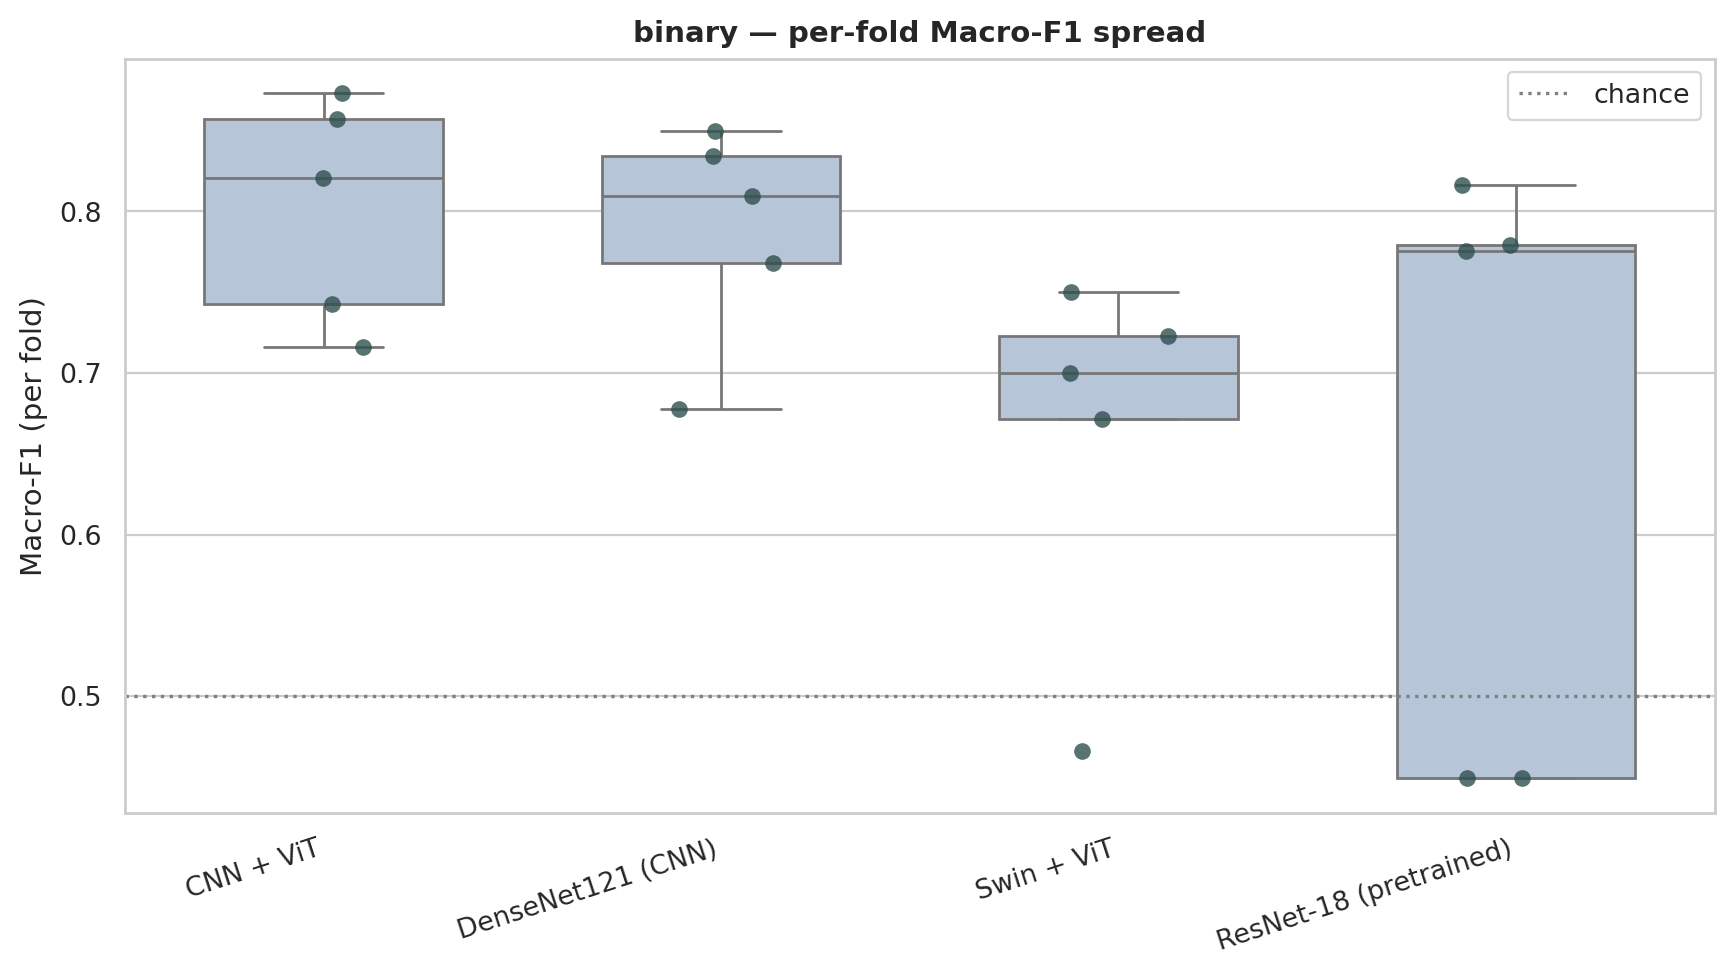
\includegraphics[width=0.49\columnwidth]{res_box_binary.png}\hfill
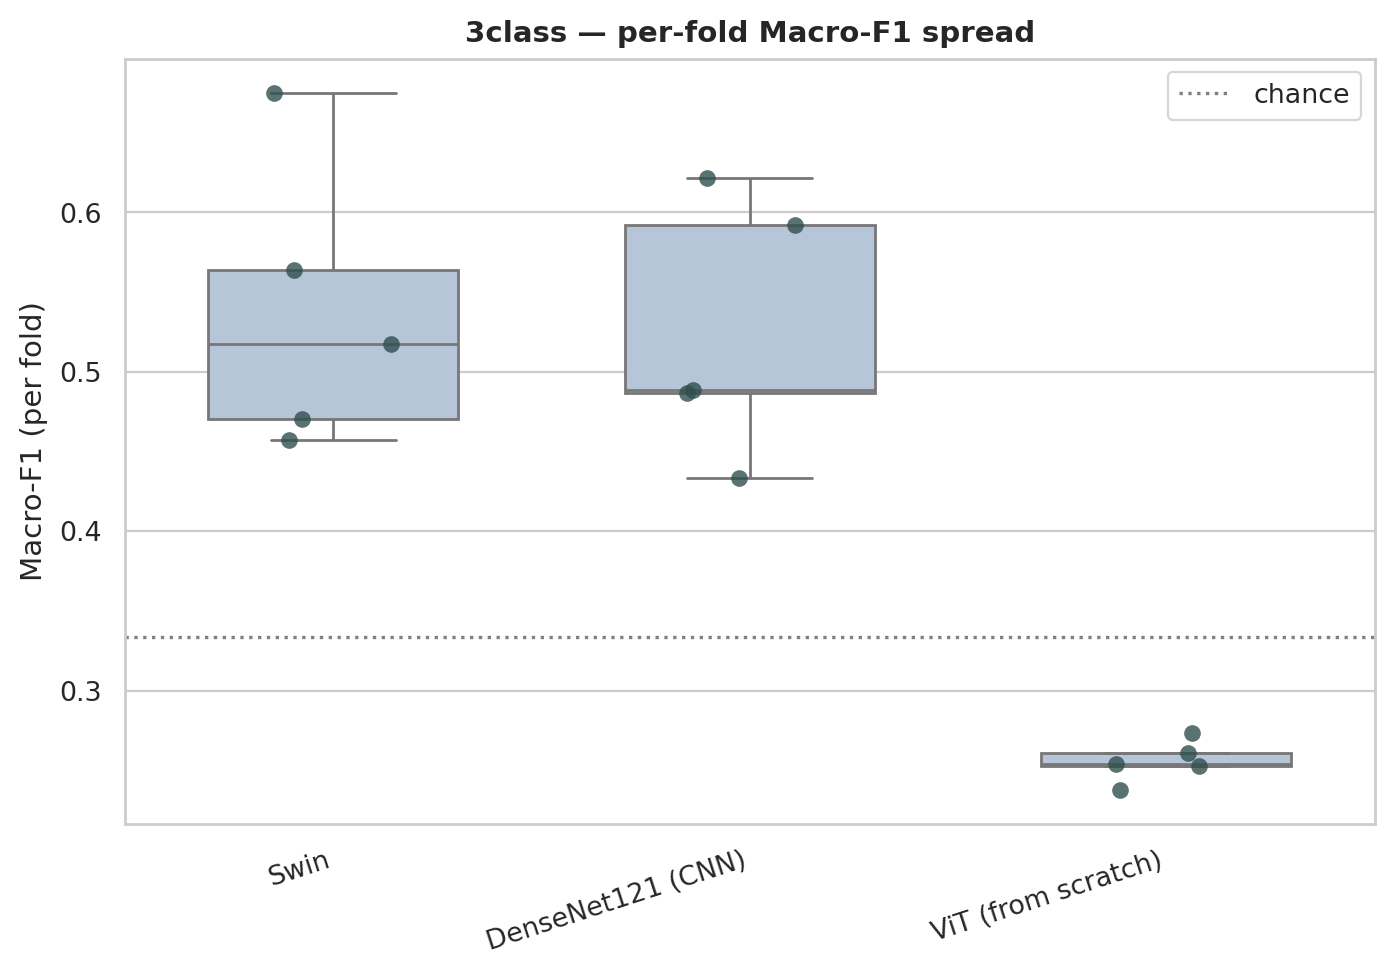
\includegraphics[width=0.49\columnwidth]{res_box_3class.png}
\caption{Per-fold macro-F1: binary (left) and three-class (right).}
\label{fig:box}
\end{figure}

\subsection{Explainability}
Fig.~\ref{fig:xai} compares the attribution methods for the binary DenseNet on one AD subject. The methods do not agree: Grad-CAM highlights frontal regions, Grad-CAM++ and Score-CAM a central peri-ventricular area, occlusion the occipital region and posterior skull, and LIME partly the scalp. Integrated Gradients is sparse on this slice. For the Swin and Swin--ViT models, group-averaged Integrated Gradients over 16 AD subjects is close to uniform across spatial thirds of the volume, and several maps fall on extra-cerebral tissue. Because the volumes are not skull-stripped, these maps cannot show that the models rely on AD-specific anatomy.

\section{Discussion}
Under subject-level evaluation our binary result ($82\%$) lies in the same regime as other subject-level 3D studies, slightly below the 85--88\% of Wen \textit{et al.}~\cite{wen2020convolutional} and the 90\% of the 138-model ensemble of~\cite{saoud2024explainable}. Our three-class result ($58\%$) is close to the 60\% reported by~\cite{saoud2024explainable}. The remaining gap is plausibly explained by our minimal preprocessing (no skull-stripping or atlas registration) and reduced $96^3$ input resolution. The 97--99\% reported by slice-level studies are not comparable.

The main finding is negative but useful. At a cohort of a few hundred subjects, a well-tuned 3D CNN is a strong baseline, and late fusion with a ViT gives no measurable gain, while transformer-only configurations are clearly weaker. Claims of hybrid superiority should therefore be supported by matched single-model baselines and paired tests on identical subject-level splits.

\textbf{Limitations.}
\begin{itemize}
    \item \emph{Incomplete model grid.} Standalone ViT and Swin were not run on the binary task, and CNN--ViT was not run on the three-class task.
    \item \emph{Statistical power.} Results come from a single seed and five folds, so differences of one or two points are within noise.
    \item \emph{Possible age confound.} AD subjects are older on average than CN subjects, and we did not run an age-only baseline.
    \item \emph{Preprocessing and explainability.} Volumes were not skull-stripped, so the explainability analysis is qualitative.
    \item \emph{External validation.} The study uses only the ADNI cohort.
\end{itemize}

\section{Conclusion}
We benchmarked six 3D models for AD classification from structural MRI under a strictly subject-level protocol. The CNN--ViT hybrid achieved the highest binary accuracy ($82.2\%$), but it was statistically tied with a from-scratch 3D DenseNet. Three-class performance was limited by MCI, and transformer-only and medically pretrained models were weaker or unstable. Future work will complete the model grid with repeated cross-validation, add skull-stripping and atlas-based ROI attribution, and validate the models on independent cohorts.

\section*{Acknowledgment}
Data collection and sharing for this project was funded by the Alzheimer's Disease Neuroimaging Initiative (ADNI). \authortodo{paste the full, current ADNI funding acknowledgement text required by the ADNI Data Use Agreement}

\vspace{2pt}
\noindent{\footnotesize Data used in preparation of this article were obtained from the Alzheimer's Disease Neuroimaging Initiative (ADNI) database (adni.loni.usc.edu). As such, the investigators within the ADNI contributed to the design and implementation of ADNI and/or provided data but did not participate in analysis or writing of this report. A complete listing of ADNI investigators can be found at: \url{http://adni.loni.usc.edu/wp-content/uploads/how_to_apply/ADNI_Acknowledgement_List.pdf}}

\bibliographystyle{IEEEtran}
\bibliography{references}

\end{document}
